\section{Statement of the Theorem}

\begin{theorem}[Kuratowski]
    \label{thr:kuratowski}
    A graph is nonplanar if and only if it has a subgraph which is a subdivision of $K_5$ or $K_{3,3}$
\end{theorem}

\begin{center}
    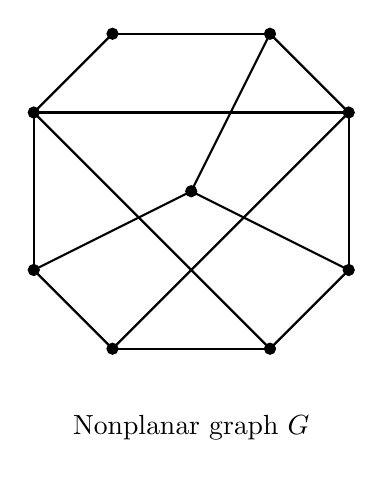
\begin{tikzpicture}
        \draw[black, thick] (0,1) -- (1,0);
        \draw[black, thick] (0,1) -- (2,2);
        \draw[black, thick] (3,4) -- (2,2);
        \draw[black, thick] (3,4) -- (1,4);
        \draw[black, thick] (0,3) -- (1,4);
        \draw[black, thick] (4,3) -- (3,4);
        \draw[black, thick] (1,0) -- (4,3);
        \draw[black, thick] (1,0) -- (3,0);
        \draw[black, thick] (3,0) -- (4,1);
        \draw[black, thick] (3,0) -- (0,3);
        \draw[black, thick] (2,2) -- (4,1);
        \draw[black, thick] (0,1) -- (0,3);
        \draw[black, thick] (4,1) -- (4,3);
        \draw[black, thick] (0,3) -- (4,3);

        \filldraw[black] (1,0) circle (2pt);
        \filldraw[black] (0,1) circle (2pt);
        \filldraw[black] (3,0) circle (2pt);
        \filldraw[black] (4,1) circle (2pt);
        \filldraw[black] (2,2) circle (2pt);
        \filldraw[black] (0,3) circle (2pt);
        \filldraw[black] (4,3) circle (2pt);
        \filldraw[black] (1,4) circle (2pt);
        \filldraw[black] (3,4) circle (2pt);

        \node at (2, -1, 0) {Nonplanar graph $G$};
    \end{tikzpicture}

\end{center}

\begin{center}
    \label{fig:G1}
    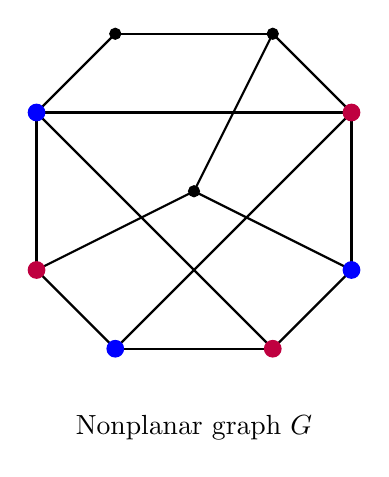
\begin{tikzpicture}
        \draw[black, thick] (0,1) -- (1,0);
        \draw[black, thick] (0,1) -- (2,2);
        \draw[black, thick] (3,4) -- (2,2);
        \draw[black, thick] (3,4) -- (1,4);
        \draw[black, thick] (0,3) -- (1,4);
        \draw[black, thick] (4,3) -- (3,4);
        \draw[black, thick] (1,0) -- (4,3);
        \draw[black, thick] (1,0) -- (3,0);
        \draw[black, thick] (3,0) -- (4,1);
        \draw[black, thick] (3,0) -- (0,3);
        \draw[black, thick] (2,2) -- (4,1);
        \draw[black, thick] (0,1) -- (0,3);
        \draw[black, thick] (4,1) -- (4,3);
        \draw[black, thick] (0,3) -- (4,3);

        \filldraw[blue] (1,0) circle (3pt);
        \filldraw[purple] (0,1) circle (3pt);
        \filldraw[purple] (3,0) circle (3pt);
        \filldraw[blue] (4,1) circle (3pt);
        \filldraw[black] (2,2) circle (2pt);
        \filldraw[blue] (0,3) circle (3pt);
        \filldraw[purple] (4,3) circle (3pt);
        \filldraw[black] (1,4) circle (2pt);
        \filldraw[black] (3,4) circle (2pt);

        \node at (2,-1,0) {Nonplanar graph $G$};
    \end{tikzpicture}

\end{center}

\begin{center}
    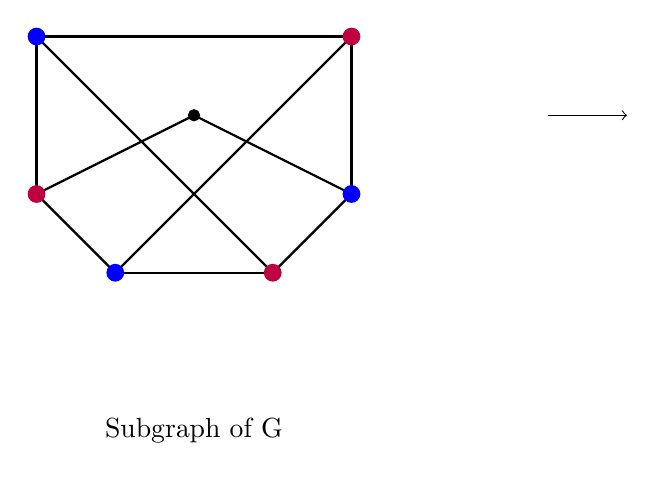
\begin{tikzpicture}
        \draw[black, thick] (0,1) -- (1,0);
        \draw[black, thick] (1,0) -- (4,3);
        \draw[black, thick] (1,0) -- (3,0);
        \draw[black, thick] (3,0) -- (4,1);
        \draw[black, thick] (3,0) -- (0,3);
        \draw[black, thick] (0,1) -- (0,3);
        \draw[black, thick] (4,1) -- (4,3);
        \draw[black, thick] (0,3) -- (4,3);
        \draw[black, thick] (0,1) -- (2,2);
        \draw[black, thick] (2,2) -- (4,1);
        \filldraw[blue] (1,0) circle (3pt);
        \filldraw[purple] (0,1) circle (3pt);
        \filldraw[purple] (3,0) circle (3pt);
        \filldraw[blue] (4,1) circle (3pt);
        \filldraw[blue] (0,3) circle (3pt);
        \filldraw[purple] (4,3) circle (3pt);
        \filldraw[black] (2,2) circle (2pt);
        \draw [-{To}] (6.5, 2) -- (7.5, 2);
        \node at (2,-2,0) {Subgraph of G};
    \end{tikzpicture}
    \hspace{2cm}
    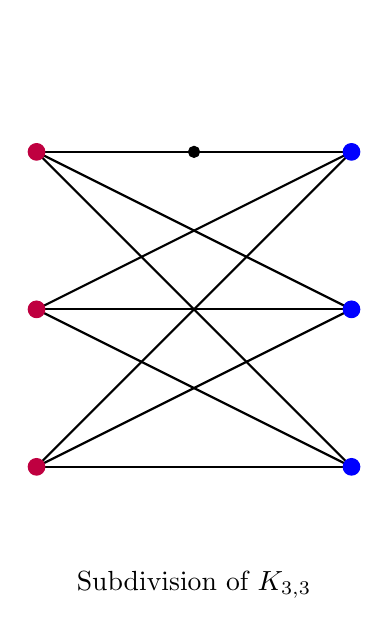
\begin{tikzpicture}
        \draw[black, thick] (8,-0.5) -- (12,-0.5);
        \draw[black, thick] (8,-0.5) -- (12,1.5);
        \draw[black, thick] (8,-0.5) -- (12,3.5);
        \draw[black, thick] (8,1.5) -- (12,-0.5);
        \draw[black, thick] (8,1.5) -- (12,1.5);
        \draw[black, thick] (8,1.5) -- (12,3.5);
        \draw[black, thick] (8,3.5) -- (12,-0.5);
        \draw[black, thick] (8,3.5) -- (12,1.5);
        \draw[black, thick] (8,3.5) -- (12,3.5);
        \filldraw[white] (10,5) circle (2pt);
        \filldraw[black] (10,3.5) circle (2pt);
        \filldraw[blue] (12,-0.5) circle (3pt);
        \filldraw[purple] (8,-0.5) circle (3pt);
        \filldraw[blue] (12,1.5) circle (3pt);
        \filldraw[purple] (8,1.5) circle (3pt);
        \filldraw[blue] (12,3.5) circle (3pt);
        \filldraw[purple] (8,3.5) circle (3pt);
        \node at (10,-2,0) {Subdivision of $K_{3,3}$};
    \end{tikzpicture}
\end{center}
